\section{The Dataset}

\begin{frame}{Problem Setting}
	\begin{block}{}
		We define the multimodal input space as the Cartesian product of $P$ modality-specific input spaces:
		\[
		\mathcal{X} = \prod_{p=1}^{P} \mathcal{X}^{(p)},
		\]
		where each modality $\mathcal{X}^{(p)}$ may represent data from distinct sources.
	\end{block}
	
\end{frame}



\begin{frame}{Toadstool 2 Dataset}
\begin{block}{}
The dataset consists of video, sensor, and demographic data collected from 10 participants playing a Super Mario Bros.
\end{block}

\vspace{-0.5em}

		\begin{columns}[T] % Top alignment
		\begin{column}{0.5\textwidth}
			\begin{center}
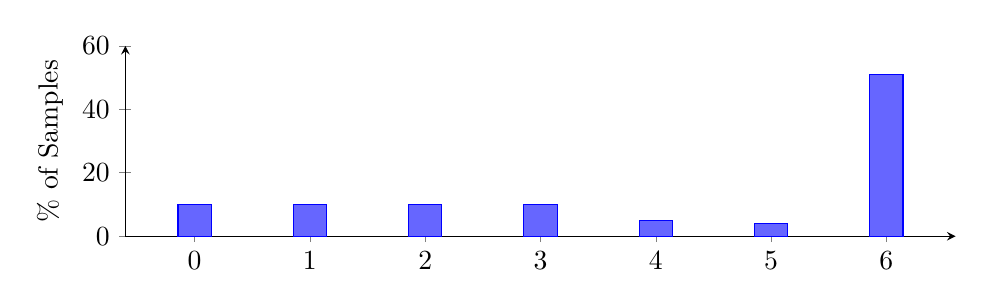
\begin{tikzpicture}
	\begin{axis}[
		width=\textwidth,
		height=4cm,
		ybar,
		bar width=12pt,
		axis x line=bottom,
		axis y line=left,
		ylabel={\% of Samples},
		symbolic x coords={0,1,2,3,4,5,6},
		xtick=data,
%		xticklabel style={rotate=0,anchor=east},
		enlarge x limits=0.1,
		ymin=0, ymax=60
		]
		\addplot+[fill=blue!60] coordinates {
			(0,10) (1,10) (2,10) (3,10) (4,5) (5,4) (6,51)
		};
	\end{axis}
\end{tikzpicture}

  \begin{columns}[t]
  \centering\footnotesize
\begin{tabular}{@{}p{0.3\textwidth} p{0.3\textwidth} p{0.3\textwidth}@{}}
	\centering 0: Anger     & \centering 1: Disgust   & \centering 2: Fear      \\
	\centering 3: Happy     & \centering 4: Sad       & \centering 5: Surprised \\
	\multicolumn{3}{c}{6: Neutral}
\end{tabular}
\end{columns}


			\end{center}
			
		\end{column}
		\begin{column}{0.5\textwidth}
		\centering
		\small
		\begin{tabular}{lcc}
		\toprule
		\textbf{Signal} & \textbf{Rate (Hz)} & \textbf{Channels} \\
		\midrule
		BVP  & 64 & 1      \\
		ACC  & 32 & 3 		\\
		EDA  & 4  & 1      \\
		HR   & 1  & 1      \\
		\bottomrule
		\end{tabular}
		
		\begin{block}{}
			20 970 sensor‐only samples (4 s windows)
		\end{block}

		\end{column}
		
	\end{columns}
\end{frame}


\begin{frame}[t]{Problem Setting}

	\begin{block}{}
		Let $\{\boldsymbol{x}^{(i)}, y^(i)\}_{i=1}^{N}$ be the train dataset, with $\boldsymbol{x}^{(i)}\in\mathcal{X}$ and $y \in \{0, 1, \dots, 6\}$. $\mathcal{X}$ is the space of vector sequences with length $T = 256$ consecutive observations, that is
		\[
		x^{(i)}
		=\bigl[\boldsymbol{x}^{(i)}_{1},\dots, \boldsymbol{x}^{(i)}_{t}, \dots,\boldsymbol{x}^{(i)}_{T}\bigr].
		\]
		$\boldsymbol{x}^{(i)}_{t}$ contain p=3 elements, one by each cnhannel denoted by x^{(i)}_{t,j}, can be either R, or be a missing valued
		
	\end{block}
\end{frame}
